
\item To determine the half life of a radioactive element, a student plots a graph of 
    \[
    \ell_n \left|\frac{dN(t)}{dt}\right| \text{ versus } t.
    \]
    Here $\frac{dN(t)}{dt}$ is the rate of radioactive decay at time $t$. If the number of radioactive nuclei of this element decreases by a factor of $p$ after 4.16 years, the value of $p$ is
    \begin{center}
        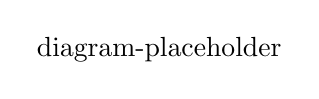
\begin{tikzpicture}
            \node at (0, 0) {diagram-placeholder};
        \end{tikzpicture}
    \end{center}
